\section{Módszerek és megvalósítás}

\subsection{NEURON idegsejt szimulációs program}
A munkánk során a Python programozási nyelvet használtuk. Az idegsejtek modellezésére pedig a NEURON programot. Szerencsére ez betölthető a Python környezetébe és így kommunikálni képes vele. Sok különböző paraméterkombinációval végzett szimuláció elvégzésénél ez nagy hasznunkra vált.

A NEURON egy szimulációs környezet idegsejtek és komplex hálózatok modellezésére. Kényelmes eszközt szolgáltat modellek építéséhez, kezeléséhez és használatához. Kifejezetten jól alkalmazható esetekhez, melyek szorosan kapcsolódnak kísérleti adatokhoz. A NEURON "motorja" különleges algoritmusokat használ annak érdekében, hogy a neurális tulajdonságokat leíró egyenleteket (melyekről később szó lesz) minél hatékonyabban oldja meg. 

Munkánk során mi két modellt építettünk, egy egykompartmentumos (ami egy neuronból áll) és egy térbelileg kiterjedt kétkompertmantumos (ami egy neuronból és egy hozzá csatlakozó dendritből áll) modellt. Valamint egy valós kísérletből származó anatómiailag részletes modellt is használtunk.

Az összes általunk használt modellt passzív idegsejti mechanizmus esetére vizsgáltuk. Ez azt jelenti, hogy az áramimpulzus hatására nem "tüzel" az idegsejt, csak passzívan folyik belsejében az áram. Kísérletileg ezt bonyolult módon csatorna blokkolókkal lehet elérni, NEURON-ban csupán beállítás kérdése.

 De hogyan is modellezünk egy biológiailag nagyon komplex idegsejtet? Meglepő módon egyszerű elektronikából ismert hálózati elemekből összerakott modell nagyon jól visszaadja az empirikus megfigyeléseket. Ezek a vezetőképességen alapuló modellek az idegsejteknek a lehetséges legegyszerűbb biofizikai reprezentációi, melyekben ion csatornákat ellenállások, illetve a kettős lipid membránt egy kapacitás helyettesíti (egy ilyen látható a~\ref{fig:fig1} ábrán). A következő szekciókban erről lesz szó, vagyis a neuronok alapvető elektromos tulajdonságairól és azok matematikai leírásáról.

\begin{figure}[!htb]
	\centering
	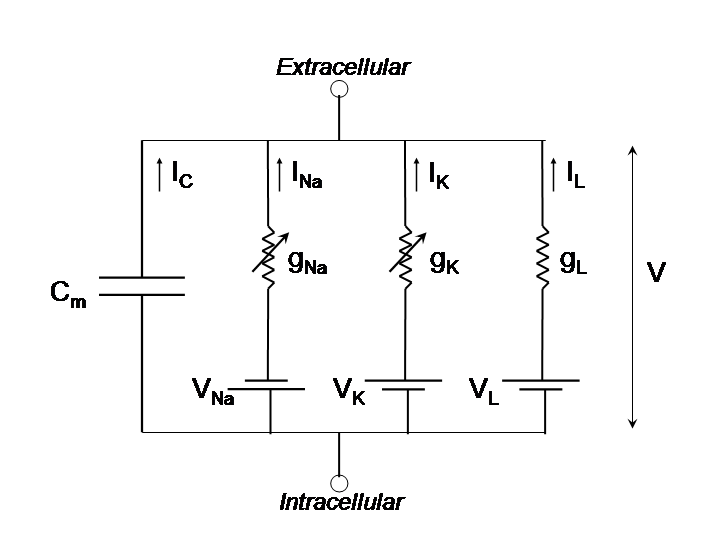
\includegraphics[width=0.7\textwidth]{./fig/Fig1.png}
	\caption[Idegsejt modell]{Példa az idegsejt konduktancián alapuló kapcsolási modelljéről. \\ \href{http://www.scholarpedia.org/w/images/e/eb/Fig1.png}{\textit{forrás: http://www.scholarpedia.org}}}
		\label{fig:fig1}
\end{figure}





\FloatBarrier
\subsection{Idegsejt modellezése}
Az idegsejtek magas ion és molekulatartalmú közegben működnek. Legtöbbször a neuron belsejében többlet negatív töltés van, ez felhalmozódik a sejtmembrán belső felületén. A külső felületére pedig az elektromos erők hatására ugyanakkora sűrűségű csak ellenkező előjelű töltés épül fel. A következőkben az idegsejtek alapvető biológiai fogalmait tárgyaljuk:

\paragraph{sejtmembrán}
A sejtmembrán egy 3-4 $nm$ vastag kettős lipid réteg, ami lényegében átjárhatatlan a legtöbb töltött molekulára nézve. A sejtmembrán ezen tulajdonsága okozza, hogy tulajdonképpen egy kondenzátorként viselkedik, mivel elkülöníti a belsejében levő és a külső töltéseket.

\paragraph{ion csatornák}
Számos típusú ion-áteresztő csatorna van beleágyazva a sejtmembránba változó sűrűséggel. Ezek bizonyos ionokat átengednek, másokat pedig nem. Részletesebben ezekre nem térünk ki, mert mi csak passzív modellekkel foglalkoztunk vizsgálataink során, aminek az a lényege, hogy ezeket a csatornákat blokkoljuk és az idegsejt (passzív) viselkedését így vizsgáljuk.

\paragraph{ion pumpák}
Az ion-pumpák tartják fenn hosszútávon a koncentrációgradienst a membrán két oldala között, energiát használva fel. Munkánkhoz ez sem kapcsolódik közvetlen.

\paragraph{membrán potenciál}
Konvenció szerint az extracelluláris potenciált rögzítjük nullára. Ennek következtében nyugalomban az idegsejt belseje negatív potenciálú. Az idegsejt akkor van nyugalomban ha a kiáramló és beáramló töltések "kioltják" egymást. A potenciál úgy változtatható meg, ha kinyitunk vagy bezárunk egy ion-csatornát, illetve ha kísérletileg áramot injektálunk a sejtbe. Mi esetünkben az utóbbit használtuk ki.
A neuron feszültsége átlagos körülmények között $-90$ és $+50$ $mV$ nagyságrendben mozog, ez teszi lehetővé, hogy az ionok a termális energiát kihasználva átlépjék a membránt. Más nagyságrendet választva nem funkcionálnának az idegsejtek. Tehát nem véletlen esett a természet választása pont erre az értékre.

Ez fontos fogalom az idegsejt leírására, mert annak épp az áramimpulzusra adott feszültségválaszát vizsgáljuk, amiből később következtetéseket vonhatunk le a modell paramétereire.



\subsubsection{Elektromos tulajdonságok}
Ebben az alfejezetben összefoglaljuk az idegsejtek alapvető elektromos tulajdonságainak a matematikai leírását.

\paragraph{membrán kapacitás}
Fentebb szó volt arról, hogy a membrán úgy viselkedik mint egy kondenzátor. Ebben az esetben az azon felhalmozódó töltést $(Q)$ a következőképp számolhatjuk ki:

\begin{equation}\label{eq:Q}
	Q = C_m V 
\end{equation}
A kapacitás $(C_m)$ azt mondja meg, hogy adott feszültség mellett mennyi töltés halmozódik fel a kondenzátor fegyverzetein, azaz jelen esetben a sejtmembránon. A kapacitás arányos a felülettel, ezért érdemes a membrán tulajdonságit jobban jellemző, felületfüggetlen mennyiség bevezetése, a specifikus membrán kapacitás:

\begin{equation}\label{eq:cm}
	c_m = \frac{C_m}{A_m}
\end{equation}
ahol $A_m$ a membrán felülete. Ez az érték tipikusan $10 \left[ \dfrac{\mu F}{cm^2}\right]$ nagyságrendbe esik.
Ha idő szerint lederiváljuk a~\ref{eq:Q} egyenlet mindkét oldalát, akkor megkapjuk a membránpotenciál megváltozását adott árambemenetre:

\begin{equation}\label{eq:dV}
	C_m \dfrac{dV}{dt} = \dfrac{dQ}{dt} = I
\end{equation}

\paragraph{membrán ellenállás}
Ahhoz is áram szükséges, hogy a membránpotenciált egy nem egyensúlyi szinten tartsuk. De ezt az áramot már a membrán ellenállás $(R_m)$ határozza meg a kapacitás helyett. Ugyanis Ohm-törvénye értelmében az $I_e$ befecskendezett áram eltolja a membrán potenciált egy $\Delta V$ értékkel:

\begin{equation}\label{eq:Rm}
	\Delta V = R_m I_e
\end{equation}
Ez a képlet csak kis $I_e$ áramok és $\Delta V$ feszültséges esetén érvényes, mivel a membrán ellenállás a feszültség függvénye egyébként.
Ennek az értéknek a variabilitása sokkal nagyobb a membránkapacitásénál. A membrán ellenállás az a membrán konduktancia (áteresztőképesség) ellentéte, ez pedig hasonlóan a membrán kapacitáshoz arányos a membrán felületével. A passzív membrán konduktancia tehát így írható fel:
\begin{equation}\label{eq:gpas}
	g_{pas} = \dfrac{1}{R_m A} = \dfrac{1}{r_m}
\end{equation}

\paragraph{membrán idő állandó}\label{par:tau}
Ha a membránkapacitást és membránellenállást összeszorozzuk akkor egy idő dimenziójú értéket kapunk. Ezt nevezzük a membrán idő állandónak, ami megadja a neurális folyamatok tipikus időskáláját:

\begin{equation}
	\tau_m = C_m R_m \approx 10-100 \left[ ms \right]
\end{equation}

\paragraph{megfordítási potenciál}
Az ionokra ható erő két fő komponensből tevődik össze, az elektromos és a kémiai potenciálból. Míg az elektromos potenciál a molekulák töltéséből fakad, addig a kémiai potenciál a koncentrációjukból. Ez a két erő tart ellen egymásnak. Egy ion-csatornát jellemző potenciál az a feszültségérték, mely meghaladása esetén az ionok ellenkező irányba kezdenek folyni rajta. Ezt nevezzük az adott csatorna megfordítási potenciáljának. Ezt úgy lehet elképzelni, hogy az adott csatorna mindig a saját megfordítási potenciálja felé próbálja terelni a feszültséget.
Annak ellenére, hogy mi a csatornákkal nem foglalkozunk ez mégis elengedhetetlen, mert a passzív konduktanciát is így modellezzük. Ennek a megfordítási potenciálja értelemszerűen a neuron nyugalmi potenciálja.

\paragraph{membrán áram}
A membrán összes csatornáján (és passzívan) átáramló áramot leosztjuk a membrán felületével, akkor megkapjuk az egységnyi felületre eső membrán áramot $(i_m)$. Mi esetünkben ez nem ion-csatornákból származik hanem csak a membránon "átszökő" töltésekből. Ezt a jelenséget a membrán passzív konduktanciájával jellemezzük és az ebből fakadó egységnyi felületre eső membránáramot a következőképpen írhatjuk le:

\begin{equation}\label{eq:im}
	i_m = g_{pas}\left( V-E_{pas}\right)
\end{equation}
ahol $g_{pas}$ a membrán passzív áteresztőképessége (konduktanciája) és $E_{pas}$ ennek a megfordítási potenciálja, ami ebben az esetben tulajdonképpen az idegsejt nyugalmi potenciálja $(E_{pas} = V_{m})$



\subsubsection{Egykompartmentumos modell}\label{sec:single-comp}
Egyetlen paraméterrel írjuk le a membránpotenciált, azaz azt tételezzük fel hogy a membrán mentén állandó a potenciálkülönbség. Ez a közelítés egy szómára (egykompartentumos modell) teljesen helytálló, mert könnyen szétterjed benne az áramimpulzus. A vékony dendritek modellezésénél (térbelileg kiterjedt modellek) viszont már térbeli függést kell feltételeznünk a membrán menti feszültségkülönbségnek (erre is van egy külön modell, a \textit{kábel egyenlet}).
A passzív egykompartmentumos modell leírásához a~\ref{eq:dV} és a \ref{eq:im} egyenleteket kell felhasználni:

\begin{equation}\label{eq:one_comp}
	c_m \dfrac{dV}{dt} = -g_{pas} \left( V-E_{pas} \right) + \dfrac{I_e}{A}
\end{equation}
ahol $I_e$ a kísérleti úton sejtbe juttatott áram. A \ref{fig:single_comp} ábrán egy általános kapcsolási rajza látható az egykompartmentumos modelleknek. Vizsgálataink során ennek a modellnek mind a $c_m$ és a $g_{pas}$ paramétereinek az inferenciájával foglalkoztunk.

\begin{figure}[!htb]
	\centering
	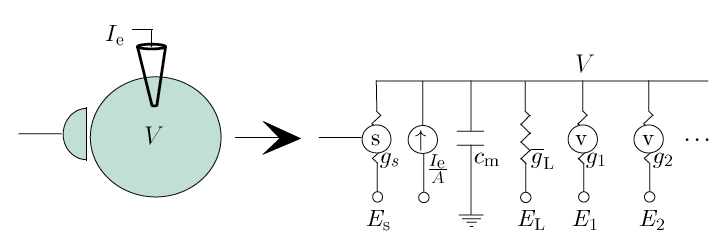
\includegraphics[width=0.7\textwidth]{./fig/single-compartment.png}
	\caption[Egykompartmentumos modell]{\cite{dayan2001theoretical} Egy általános egykompartmentumos modell, melyen a ion-csatornák mellett még egy szinaptikus kapcsolat is van.}
	\label{fig:single_comp}
\end{figure}



\FloatBarrier
\subsubsection{Térbelileg kiterjedt modellek}\label{sec:multi-comp}
A térbelileg kiterjedt modelleknél már nem tehetjük fel, hogy a membrán mentén a potenciál konstans. Ez úgy orvosolhatjuk, hogy több elemből építjük fel az idegsejtet, melynek az egyes kompartmentumjaiban rögzítjük a potenciált. Minél több részre osztjuk a sejtet, annál részletesebben tudjuk leírni a viselkedését. Ezt a folyamatot, vagyis a modellezés különböző szintjeit mutatja be szemléletesen a \ref{fig:multi_comp} ábra. Ez matematikailag összekapcsolt egykompartmentumos modellekkel írható le a következő módon (passzív idegsejt esetén):

\begin{equation}\label{eq:multi_comp}
	c_m\dfrac{dV_\mu}{dt} = -g_{pas}\left(V - E_{pas}\right) + \dfrac{I_e^\mu}{A_\mu} + g_{\mu,\mu+1}\left(V_{\mu+1}-V_\mu \right) + g_{\mu,\mu-1}\left(V_{\mu-1}-V_\mu \right)
\end{equation}
ahol $I_e^\mu$ az adott $\mu$-edik kompartmentumba befecskendezett áram, $V_\mu$ a $\mu$-edik kompartmentum membrán potenciálja, $A_\mu$ a $\mu$-edik kompartmentum felülete. Ennek megfelelően $V_{\mu+1}$ és $V_{\mu-1}$ a jelenlegi komparmentumhoz csatlakozó másik kompartmentumok feszültségei. $g_{\mu,\mu+1}$ és $g_{\mu,\mu-1}$ a csatolási tényező, áteresztőképesség a kompartmentumok között. Ez felírható a következőképp is:

\begin{equation}\label{eq:Ra}
	g_{\mu,\mu+1} = \dfrac{1}{R_a^{\mu,\mu+1} A_\mu}
\end{equation}
ahol $R_a$ az axiális ellenállás. Inferencia során ezt a paramétert is becsültük, a kompartmentumok között állandónak tekintve ezt az értéket: 
\[ R_a^{\mu,\mu-1} = R_a^{\mu,\mu+1} = ... = R_a \]
Egy ilyen modellnek az általános kapcsolási rajza a \ref{fig:multi_comp_model} ábrán látható. 

Mi egy úgynevezett \textit{Ball and Stick} modellt építettünk vizsgálataink során, ami egy szómához kapcsolódó dentrit esetét reprezentálja. Ezen kívül vizsgáltunk egy kísérletből származó bonyolult három dimenziós morfológiát is. Erről a NEURON program segítségével előállított rajz a~\ref{fig:morph} ábrán látható.


\begin{figure}[!htb]
	\centering
	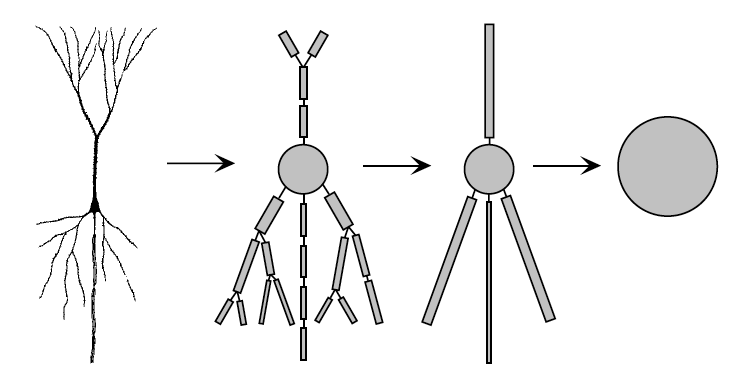
\includegraphics[width=0.7\textwidth]{./fig/multi-compartment.png}
	\caption[Többkompartmentumos modellezés]{\cite{dayan2001theoretical} Egy idegsejt különböző szintű kompartmentális modellezése. Jobbra haladva egyre inkább leegyszerűsítve írjuk le a sejtet.}
	\label{fig:multi_comp}
\end{figure}

\begin{figure}[!htb]
	\centering
	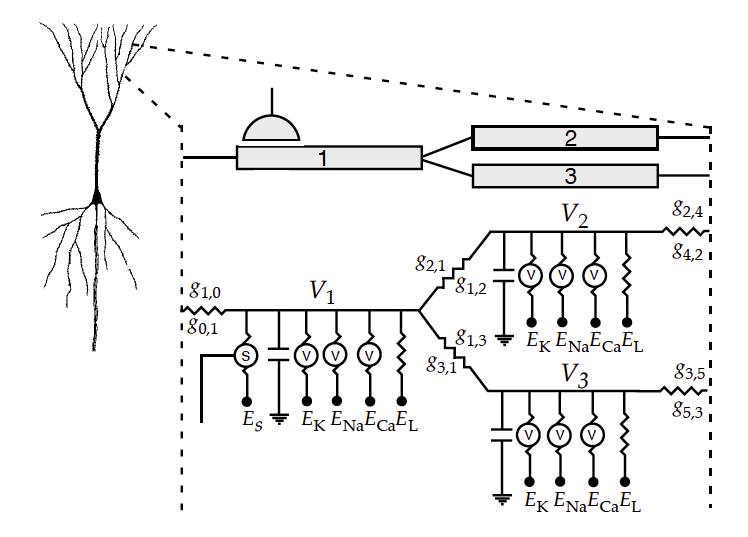
\includegraphics[width=0.7\textwidth]{./fig/multi-comp-model.png}
	\caption[Többkompartmentumos modell]{\cite{dayan2001theoretical} Egy kiterjedt idegsejt többkompartmentumos (általános) modelljének kapcsolási rajza.}
	\label{fig:multi_comp_model}
\end{figure}

\begin{figure}[!htb]
	\centering
	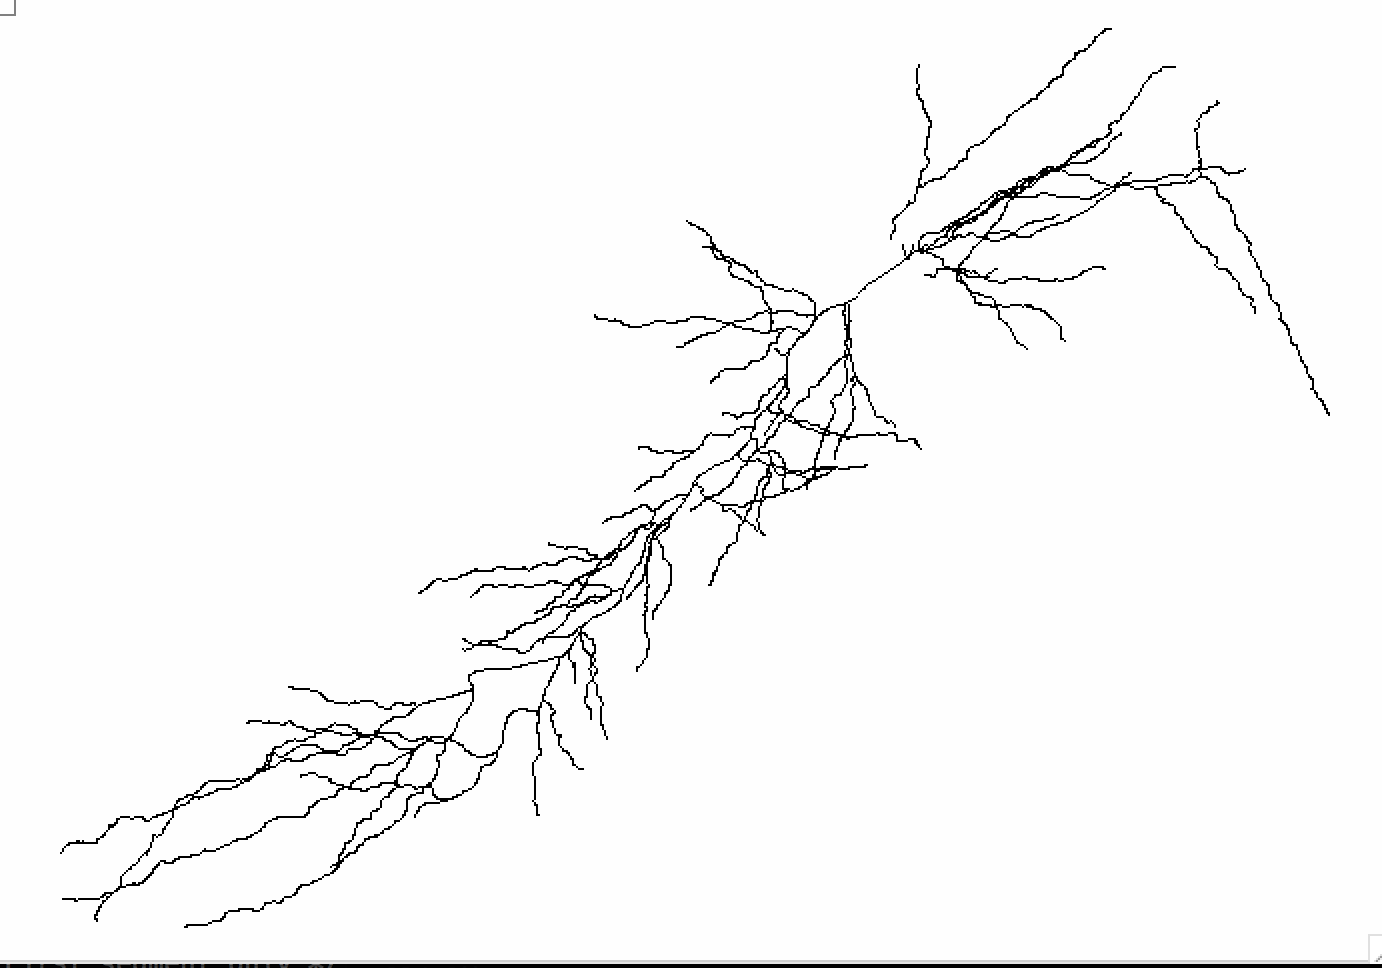
\includegraphics[width=0.5\textwidth]{./fig/morph.png}
	\caption[Kísérletből származó morfológia]{Egy valós idegsejt NEURON programba töltött modellje}
	\label{fig:morph}
\end{figure}





\FloatBarrier
\subsection{Eloszlásbecslés Bayesiánus formalizmussal}\label{sec:bayes}
Célunk az idegsejt modellezés eszközeivel adott mérési eredmények alapján különböző paraméterek poszterior eloszlását meghatározni a kiválasztott sejttípuson belül, mivel ez sok lényeges információt hordozhat (paraméterek várható értéke, közöttük levő korreláció, becslés információtartalma...). Erre a problémakörre jól alkalmazható a Baysiánus inferencia módszere, amit a következőkben tárgyalunk.

\paragraph{valószínűségi változók}
A modell paramétereire úgy tekintünk, mint valószínűségi változókra $(\xi)$, melyekhez eloszlásfüggvényt szeretnénk rendelni.

\paragraph{poszterior eloszlás}
Paraméterek poszterior eloszlását szeretnénk meghatározni adott kísérleti eredmények mellett.
Elsődleges szempont tehát, hogy legyenek kísérleti eredményeink (például a mi esetünkben passzív idegsejtek válasza áramimpulzus hatására). Valamint jellemezni kell valamilyen módon, hogy az adatok mennyire támasztják alá a modellünk adott paraméterek melletti helyességét. Ezeken felül hasznos, ha vannak előzetes ismereteink a becsülendő paraméterekről. Ezen összetevőkből egy poszterior eloszlás készíthető a következő módon:

\begin{equation}\label{eq:bayes}
P_i(\xi|D) = \dfrac{P_i(D|\xi)P(\xi)}{\int P_i(D|\xi)P(\xi)d\xi}
\end{equation}
ahol $D$ a kísérleti adat, $i$ az áramimpulzusra adott választ jelöli és $\xi$ pedig a modellparamétereinket.
\begin{itemize}
	\item $P_i(\xi|D)$: Ez a poszterior eloszlás, a keresett paraméterek valószínűségi eloszlása a mérési adatok figyelembevétele után.
	\item $P_i(D|\xi)$: Ez a likelihood eloszlás, azt jellemzi mennyire valószínű ezeknek az adatoknak a mérése, ha az adott paraméterbeállítással vett modellünket vesszük igaznak. A következő pontban ezt részletesen tárgyaljuk.
	\item $P(\xi)$: Ez a prior eloszlás, előzetes ismereteink a paraméterekről. Úgy is felfoghatjuk, hogy ezt az eloszlást frissítjük az új adatok függvényében, így keletkezik a poszterior eloszlás. Új méréseket végezve ez a folyamat tovább iterálható.
	\item $\int P_i(D|\xi)P(\xi)d\xi$: Ez csupán a normálási faktor. Annak a következménye, hogy a valószínűségi eloszlásoknak normáltnak kell lenniük, így teljes tartományra vett integráljuknak egy. A normálási faktor ezzel a tulajdonsággal ruházza fel a poszterior értékünket, aminek következtében teljes értékű valószínűségi eloszlás lesz.
\end{itemize}

\paragraph{marginalizálás}
Előfordulhat, hogy néhány paraméterre nem vagyunk kíváncsiak (például csak azért vettük be a modellünkbe, hogy lássuk mennyire torzítja el a többi paraméter eloszlását). Tegyük fel, hogy $\xi$ a cél paramétereink, de a modellt kiterjesztettük további $\theta$ változóval, aminek viszont az eloszlása nem érdekel. Továbbra is $P_i(\xi|D)$ meghatározása a feladat.  A likelihood viszont ekkor ilyen formában írható fel:
\[
P_i(D|\xi, \theta)
\]
A "felesleges" változókat egyszerűen kiintegrálva (a priorjaival együtt) visszakapjuk a~\ref{eq:bayes}-es egyenletben szereplő likelihood formát:

\begin{eqnarray}\label{eq:marginalize}
P_i(D|\xi) = \int P_i(\xi, \theta)P(\theta)d\theta
\end{eqnarray}
Viszont ez nem feltétlen fogja ugyan azt az eredményt szolgáltatni, ugyanis a paraméterek között komplex összefüggések lehetnek.

\paragraph{numerikus implementálás}
Numerikusan nem lehetséges egzaktul folytonos függvények kezelése. Mégis diszkrét eloszlások bevezetése helyett, \textit{kvázi-folytonosnak} tekintjük őket és alkalmazzuk rá a numerikus eljárásokat, mintha folytonosak lennének.





\subsection{Likelihood függvény}\label{sec:likelihood}
Előző fejezetben már volt szó a likelihood függvény szerepéről. Most arról lesz szó, hogy mi ezt milyen módszerrel konstruáltuk meg.

Azt szeretnénk elérni, hogy a kísérleti adatokat összemérjük a modellünk eredményeivel. Ehhez megvan a modellünk a Neuron programban és tegyük fel, hogy kísérleti adataink is vannak. Össze kell hasonlítanunk a kísérleti eredményünket a modellünkből kinyert eredménnyel. Az eltérést szemlélteti a \ref{fig:compare} ábra, ahol a zöld függvény az adott paraméterek melletti modellünk eredménye.
\begin{figure}[!htb]
	\centering
	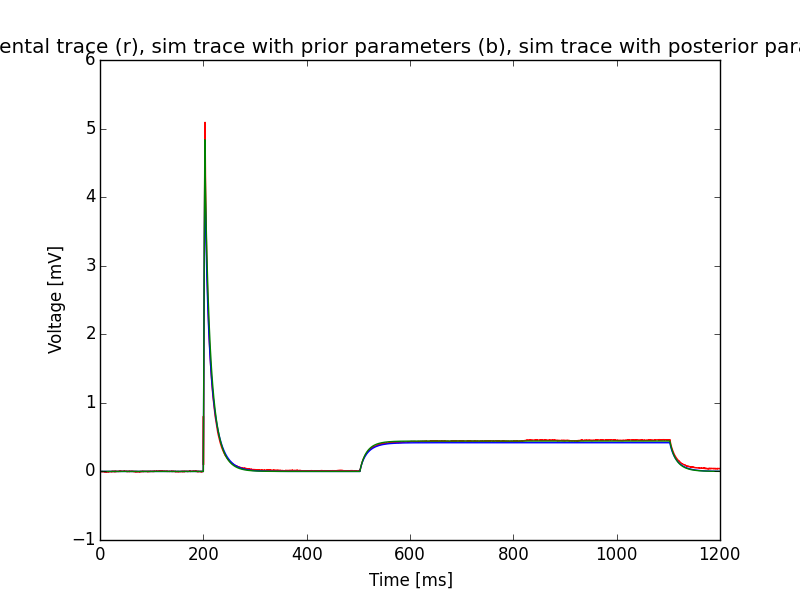
\includegraphics[width=0.7\textwidth]{./fig/compare.png}
	\caption[Kísérletből és szimulációvól származó adatok]{A kísérleti adatokat jelöljük pirossal, a szimulációból eredőt pedig zölddel. Az idő függvényében $(ms)$ van kirajzolva az idegsejt áramimpulzusokra adott feszültségválasza $(mV)$.}
	\label{fig:compare}
\end{figure}
Ezekhez a paraméterekhez (amik a \ref{fig:compare} ábrán a zöld függvénymenetet eredményezték) szeretnénk egy valószínűségi értéket társítani, ami jellemzi a kísérleti adatokkal való egybevágóságot. Egy jó megközelítés ennek a megvalósítására, hogy a adatpontok eltérésének a nagyságát egy exponenciálisan lecsengő függvénybe rakjuk. Ez ugyanis nagy eltérések mellett kis értékeket fog adni, közel megegyező pontok esetén (ahol nincs eltérés) pedig nagyobb értéket. Következő pontokban ezt öntjük matematikai formába:


\subsubsection{Normál eloszlás}
A függvény alakjának célszerű a normál (gauss) eloszlást választani, amely egy változó esetén a következő módon néz ki:

\begin{equation}\label{eq:gauss}
	N\left(x|\mu=0, \sigma^2\right) = \dfrac{1}{\sqrt{2\pi \sigma^2}}e^{-\dfrac{\left(x-\mu\right)^2}{2\sigma^2}}
\end{equation}
mivel $\mu$ értékétől független a szolgáltatott eredmény, ezért azt tetszőlegesen megválaszthatom, jelen esetben az egyszerűség kedvéért nullának. 

\paragraph{általános alak}
Mivel a függvényalakunk (\ref{fig:compare}) sok pontból áll, érdemes az általános $D$ dimenziós alakot bevezetni:
\begin{equation}\label{eq:gaussD}
	N\left(\vec{x}|\vec{\mu}=\vec{0}, \underline{\underline{ \Sigma }}\right) = \dfrac{1}{\left(2\pi\right)^{D/2} \sqrt{\det \underline{\underline{ \Sigma }}}}\exp\left[-\dfrac{1}{2}\left(\vec{x}-\vec{\mu}\right)^T \underline{\underline{ \Sigma }}^{-1}\left(\vec{x}-\vec{\mu}\right)\right]
\end{equation}
ahol $\underline{\underline{ \Sigma }}$ a valószínűségi változók kovariancia mátrixa. Ennek a főátlójában a szórás négyzetek helyezkednek el, a többi helyen pedig a megfelelő kereszt tagok. Ennek következében ez egy szimmetrikus mátrix. 

\paragraph{független eset}
Speciális eset ha a mátrixnak csak a főátlójában helyezkednek el tagok, ami azt jelenti, hogy a pontok függetlenek, így szétválik a valószínűségi eloszlásfüggvény az egydimenziós esetek (\ref{eq:gauss}) szorzat alakjára (legyen a szórás is ugyan az):
\begin{equation}\label{eq:gauss_independent}
		N\left(\vec{x}|\vec{\mu}=\vec{0}, \underline{\underline{ \Sigma }}\right) = N\left(x_1, x_2, \ldots, x_n| \sigma^2\right) = N\left(x_1| \sigma^2\right)\cdot N\left( x_2| \sigma^2\right) \cdot \ldots \cdot N\left( x_n| \sigma^2\right) = 
\end{equation}

\begin{equation}
		= \dfrac{1}{\sqrt{2\pi \sigma^2}}\exp \left[-\dfrac{x_1^2}{2\sigma^2}\right] \cdot \dfrac{1}{\sqrt{2\pi \sigma^2}}\exp\left[-\dfrac{x_2^2}{2\sigma^2}\right] \cdot \ldots \cdot \dfrac{1}{\sqrt{2\pi \sigma^2}}\exp \left[-\dfrac{x_n^2}{2\sigma^2}\right] =
\end{equation}

\begin{equation}
	=  \left(\dfrac{1}{\sqrt{2\pi \sigma^2}}\right)^n \exp \left[-\dfrac{x_1^2 + x_2^2 + \ldots + x_n^2}{2\sigma^2}\right]
\end{equation}


\subsubsection{Likelihood megkonstruálása}
Most pedig tekintsük át, hogyan is alkalmazható a gyakorlatban ez az elmélet. A \ref{eq:gaussD} képletnek kell szolgáltatni egy $\vec{x}$ vektort és egy $\underline{\underline{\Sigma}}$ mátrixot, eredményül pedig egy skalárt ad, ami az adott paraméterkombináció jóságát jellemzi. Az előbbi a pontbeli eltérésekből (\ref{fig:compare}) gyártott vektor, az utóbbi pedig a kísérletből fakadó zaj autokorrelációs függvénye által meghatározott kovariancia mátrix, amiről később lesz szó.
Ha az adatpontokat függetleneknek, vagy függőknek tekintjük, különböző módon kell eljárnunk:
 
 \paragraph{független eset}
Azt már említettük is fentebb, hogy független pontok esetében szorzat alakra bomlik a megoldás. Ekkor a likelihood értékek konstruálását a következő lépések írják le:
\begin{enumerate}\label{meth:independet}
	\item Adott paraméterkombinációval lefuttatjuk a szimulációt a NEURON program segítségével.
	\item Megnézzük a kísérleti és a szimulációs adatok négyzetes eltérését minden pontban és összegzünk is erre.
	\item Az összegzett értéket megszorozzuk $-1/(2 \sigma^2)$ -tel, ahol $\sigma$ a független zaj szórása.
	\item Ezt elvégezzük az összes lehetséges paraméterkombinációra és tároljuk az eredményt. Numerikus okokból érdemes a legnagyobb értéket kivonni az összesből.
	\item Végül ezt exponencializálva megkapjuk az összes paraméterbeállítás likelihood értéket $\Rightarrow P_i(D|\vec{\xi})$.
\end{enumerate}
Tulajdonképpen nem csinálunk mást, mint a \ref{eq:gauss_independent} képlet exponensébe a négyzetes eltéréseket helyettesítjük (a normálási faktorral elegendő csak a legvégén, a poszterior eloszlás megalkotásánál foglalkozni). Ezzel egy gauss jellegű likelihood függvényt kapunk a vizsgált paramétereink tartományai fölött, ami egy kísérletből származó valószínűséget rendel az egyes paraméterértékekhez.

\paragraph{átalános eset}
Általános nem független esetben az előző lépések így módosulnak:
\begin{enumerate}\label{meth:dependet}
	\item Adott paraméterkombinációval lefuttatjuk a szimulációt a NEURON program segítségével.
	\item Megnézzük a kísérleti és a szimulációs adatok négyzetes eltérését minden pontban és ezeket egy vektorban tároljuk.
	\item A zaj inverz kovariancia mátrixát megszorozzuk balról és jobbról is az előbbi különbségvektorral és ezt egy további $-1/2$ faktorral.
	\item Ezt elvégezzük az összes lehetséges paraméterkombinációra és tároljuk az eredményt. Numerikus okokból érdemes a legnagyobb értéket kivonni az összesből.
	\item Végül ezt exponencializálva megkapjuk az összes paramétermegválasztás likelihood értéket $\Rightarrow P_i(D|\vec{\xi})$.
\end{enumerate}
Tulajdonképpen nem csinálunk mást, mint a \ref{eq:gaussD} képlet exponensébe a négyzetes eltérésvektorokat és a zaj inverz kovariancia mátrixát helyettesítjük (numerikusan itt sem kell törődni a normálással). Ezzel egy gauss jellegű likelihood függvényt kapunk a vizsgált paramétereink tartományai fölött, ami egy kísérletből származó valószínűséget rendel a paraméterértékekhez.

Azt hogy az adatpontok milyen módon függnek és ekkor mi lesz a \ref{eq:gaussD} normál eloszlásban szereplő kovariancia mátrix, a kísérleti zaj határozza meg, ha a kísérletből nem származna zaj és a kinyert adatok determinisztikusak lennének, akkor ezzel nem kellene foglalkoznunk (függetlenek lennének nulla szórással). A problémakörnek ez is egy fontos része, a következőkben erről lesz szó részletesebben.




\FloatBarrier
\subsection{Zajmodellek}\label{sec:noise}
A \ref{sec:bayes} fejezetben bevezettünk egy valószínűségi leírást, aminek fontos alkotóeleme a kísérleti adatsor $D$ (mi esetünkben ez a passzív idegsejt áramimpulzusra adott feszültségválasza). Minden kísérletnél elkerülhetetlen tényező a zajok megjelenése. Tegyük fel, hogy van egy determinisztikus eredmény $(D^*)$, amire kísérleti zajt rakva $(z)$ kapjuk meg a valódi mért adatokat $(D)$. 
\[
D = D^* + z
\]
Ez azt jelenti, ha jól ismerjük a kísérletből fakadó zajt, akkor egyrészt szintetikus kísérleti adatokat tudunk előállítani, másrészt pontosabban elvégezhető az inferencia, mivel a likelihood függvényben megjelenő kovarianciamátrixot épp a zaj $(z)$ autokorrelációs függvénye határozza meg, így paraméterbecslésnél a zajt is figyelembe vesszük.

Szintetikus adatok előállításával mi is foglalkoztunk, mivel a statisztikus modellünket kezdetben ily módon gyártott "kísérleti" adatokra alkalmaztuk.

Kétfajta zajmodellel dolgoztunk: egy igen primitív független zajjal, a fehér zajjal, valamint egy sokkal realisztikusabb és korrelálóval, a színes zajjal. Ezekről lesz szó a következő pontokban, de előbb nézzük meg hogyan is áll elő a kovariancia mátrix.

\subsubsection{Kovariancia mátrix}
Két valószínűségi változó kovarianciája:
\begin{equation}\label{eq:cov}
	cov(\xi,\chi) = E\left[(\xi-E[\xi])(\chi-E[\chi])\right] = E[\xi\chi] - E[\xi]E[\chi]
\end{equation}
Ahol $E$ (expected value, szokás jelölés még: $<x>$, $\overline{x}$) a várható értéket jelöli. (Kiszámítani úgy kell, hogy a valószínűségi változót integrálom a sűrűségfüggvényével az egész téren.) Tulajdonképpen azt jellemzi, hogy a két valószínűségi változó mennyire mozog együtt. Érdemes még tovább elemezni a $\chi=\xi$ esetet:
\begin{equation}\label{eq:cov_var}
	cov(\xi,\xi) = <\xi^2> - <\xi>^2 = \sigma_\xi^2 = var_\xi
\end{equation}
ez épp a $\xi$ valószínűségi változó szórás négyzete, azaz varianciája. 
Legyen $n$ darab valószínűségi változónk: $x_1, x_2, \ldots , x_n$. Ekkor ezeknek a kovariancia mátrixát a következőképp definiáljuk:
\begin{equation}\label{eq:covmat}
	\Sigma_{ij} = cov(x_i, x_j)
\end{equation}
Ez a mátrix szimmetrikus, mivel a \ref{eq:cov} kifejezés invariáns a változócserére, valamint a főátlójában a változók szórás négyzetei szerepelnek \ref{eq:cov_var} kifejezés értelmében. Tehát ez a mátrix tartalmazza a valószínűségi változók szórás négyzeteit és minden egyes tag minden másikkal vett kovarianciáját.

A mi esetünkben a valószínűségi változók az összes időpillanatban vett eltérések a függvényértékeink között. Ezeknek a valószínűségi változóknak (adott időpillanatokban kinyert mérési eredmény) egymással vett korrelációját csak a kísérleti zaj határozza meg. A következő pontokban ezekkel a zajmodellekkel foglalkozunk.

\subsubsection{Fehér független zaj}
\paragraph{tulajdonságai}
Tegyük fel hogy a kísérleti zajunk Gauss fehér zaj $(z = g_w)$. Ennek a következő tulajdonságai vannak:
\begin{equation}
	<g_w(t)> = 0
\end{equation}
vagyis várható értéke nulla és
\begin{equation}
	<g_w(t)g_w(s)> = 2\sigma^2\delta(t-s)
\end{equation}
időben független, nem korrelál önmagával a zajfüggvény, mivel az autokorrelációs függvénye egy Dirac-delta függvény (a képletben $\delta(x)$ jelöli a Dirac-delta függvényt, ami mindenhol nulla csak $x=0$ ban végtelen ). Ez azt jelenti, hogy ilyen zajmodellek esetén elég a független esetekben érvényes likelihood függvény előállítás módszert bevetni (\ref{meth:independet}), ami sokkal kevésbé számításigényes (egy teljes kovariancia mátrix helyett elegendő csupán a zaj szórásával számolni).

\paragraph{kovariancia mátrixa}
A fehér zaj tulajdonságait visszahelyettesítve a \ref{eq:cov} képletbe, a kovarianciamátrix elemei így alakulnak:
\begin{equation}
	\Sigma_{ij} = 2\sigma^2 \delta_{ij}
\end{equation}
ahol $\delta_{ij}$ a Kronkecker-delta kifejezés, $\sigma$ pedig a zaj szórása. Ez azt jelenti, hogy a mátrix diagonálisában szerepelnek a szórások és visszakaptuk a független esetet.

\paragraph{előállítása}
Ilyen zajt egy normál eloszlásból való véletlen mintavételezéssel generálhatunk (az így kapott zaj szórása megegyezik a normál eloszlás $\sigma$ paraméterével). A Python Numpy csomagjában található egy ilyet megvalósító függvény, amit segítségül hívtunk. Egy ilyen zaj látható a \ref{fig:white} ábrán.

\begin{figure}[!htb]
	\centering
	\includegraphics[width=0.8\textwidth]{./fig/white.png}
	\caption[Fehér zaj]{Determinisztikus függvény és arra rakott nagy szórású fehér zaj.}
	\label{fig:white}
\end{figure}


\FloatBarrier
\subsubsection{Exponenciálisan korreláló színes zaj}
A kísérleti zaj egy sokkal realisztikusabb modellje az önmagával időben exponenciálisan korreláló úgynevezett színes zaj. Ez a zajmodell jobban leírja az elektrofiziológiai kísérletek során keletkező zajt. 

\paragraph{tulajdonságai}
Tegyük fel hogy a kísérleti zajunk színes zaj $(z = \epsilon)$. Ennek a következő tulajdonságai vannak:
\begin{equation}
<\epsilon(t)> = 0
\end{equation}
vagyis várható értéke nulla és
\begin{equation}
<\epsilon(t)\epsilon(s)> = D\lambda \exp(-\lambda|t-s|)
\end{equation}
önmagával exponenciálisan korrelál, mivel az autokorrelációs függvénye exponenciálisan lecsengő. Ebben a képletben $D$ az amplitúdó és $\lambda$ pedig a karakterisztikus idő, azt mondja meg milyen gyorsan cseng le a korreláció a vizsgált pontok távolodása esetén. 

Korreláló adatpontok esetén a \ref{meth:dependet} metódust kell követni. Az ehhez szükséges kovarianciamátrixot a zaj autokorrelációs függvénye határozza meg.

\paragraph{kovariancia mátrixa}
A színes zaj tulajdonságait visszahelyettesítve a \ref{eq:cov} képletbe, a kovarianciamátrix elemei így alakulnak:
\begin{equation}\label{eq:covmat_col}
	\Sigma_{ij} = D\lambda e^{\lambda |t_i - t_j|}
\end{equation}
ahol $t_i$ az $i$-edik időpillanat.

\paragraph{előállítása}
Egy ilyen tulajdonságú zaj előállítása nem triviális feladat. Ronald F. Fox és Ian R. Gatland által kifejlesztett metódust \cite{PhysRevA.38.5938} implementáltuk Pythonban.
A \ref{fig:colored} ábrán látható két determinisztikus függvény, amire színes zajt raktunk. Látható módon ez tényleg korrelál önmagával. Ez a zaj a következő paraméterekkel állt elő:
\begin{itemize}
	\item $D = 30$
	\item $\lambda = 0.1$
\end{itemize}

\begin{figure}
	\hfill
	\subfloat[Színe zaj A]{{\includegraphics[width=0.45\textwidth]{./fig/colored1.png} }}%
	\hfill
	\subfloat[Színes zaj B]{{\includegraphics[width=0.45\textwidth]{./fig/colored2.png} }}%
	\hfill
	\caption[Színes zaj]{2 ábra a (nagy amplitúdójú) színes zajról, ami rárakódott a determinisztikus (piros) függvényre. Passzív idegsejt áramimpulzusra adott feszültségválasza látható a képen (az idő függvényében a feszültség).}%
	\label{fig:colored}
\end{figure}

\FloatBarrier